	\section{Durchführung}
  \begin{figure}[H]
    \center
    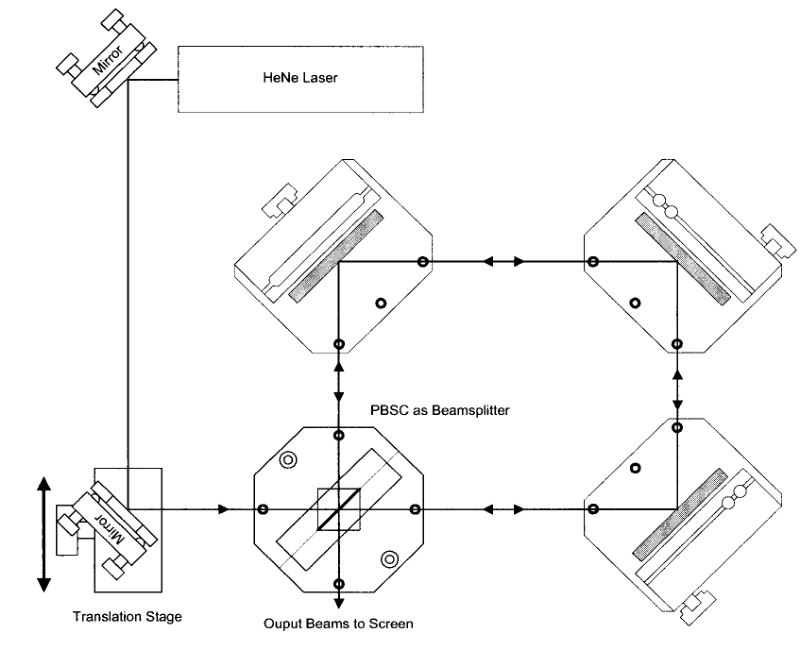
\includegraphics[width=\textwidth]{./plots/Versuchsaufbau.JPG}
    \caption{Aufbau des Sagnac-Interferometers\cite{Anleitung}}
		\label{aufbau}
	\end{figure}
 In der Abbildung \ref{aufbau} ist der generelle Aufbau des Sagnac Interferometers zu sehen. Hinter dem PBSC aus der Abbildung wird
  zur Messung der Interferenzmuster noch ein weiterer PBSC zur Teilung des Strahls auf 2 Photodioden eingebaut. Die Strahlen werden ausserdem in eine Polarisationsebene projeziert, wodurch die Interferenz gewährleistet wird.
	Die Signale der Dioden werden auf einem Oszilloskop von einander subtrahiert und als Differenzsignal visualisiert.
  Zur zusätzlichen Justierung wird der HeNe-Laserstrahl vor dem Auftreffen auf den PBSC noch über 2 Spiegel geleitet. Durch den linken unteren Spiegel kann die Aufteilung des Strahls in hin- und rückläufigen
  Strahl bewirkt werden, was für die späteren Messungen von Nöten ist, indem der ein wenig entlang der Vertikalen zwischen den ersten zwei Spiegeln
	in Abb. \ref{aufbau} verschoben wird. Dies führt dazu, dass der einlaufende Strahl nicht mehr exakt zentrisch auf den ersten PBSC trifft, sondern in der Horizontalen verschoben. Hierdurch überlagern sich die zwei gegenläufig durchs Interferometer laufenden Strahlen nicht mehr. Zur korrekten Justierung des Strahls auf die Spiegel werden ausserdem Lochblenden verwendet.\\
  Bevor mit der Messung der Intensitätsmaxima und Minima begonnen werden kann, werden nun die Strahlen im Interferometer korrekt auf den zweiten, um 45° gegen die horizontale geneigten PBSC ausgerichtet. Dieser projeziert die zwei orthogonal zueinander polarisierten Strahlen in eine Polarisationsebene, wodurch Interferenzeffekte in beiden aus diesem austretenden Strahlen auftreten.\\
  Anschließend werden die Plättchen in das Interferometer gebracht. Nun wird der Polarisationsfilter, welcher vor Punkt 1 in Abbildung \ref{aufbau} positioniert ist,
  in 10° Schritten gedreht.
	Aus dem auf dem Oszilloskop sichtbaren Referenzsignal lassen sich nun die maximalen und minimalen Intensitäten ablesen, welche entstehen, wenn
  man die Plättchen im Interferometer um einen Winkel im Strahl kippt. Aus den gemessenen Daten wird in der Auswertung der Kontrast errechnet.\\
  \\
  Im zweiten Teil des Versuchs soll der Brechungsindex der zuvor bereits verwendeten Plättchen ermittelt werden. Die Plättchen werden nun senkrecht zur Strahlachse so im Strahl positioniert, dass sie bei Blick von oben auf den optischen Tisch um 10° zueineander geneigt erscheinen.
  Anschließend wird die Anzahl der Interferenzmaxima bei einer Rotation um 10° senkrecht zur Strahlebene in 1° Schritten gemessen.\\
  \\
  Im letzten Teil des Versuchs wird statt der Plättchen eine Gaszelle in einen der beiden umlaufenden Laserstrahlen im Interferometer geschoben und mithilfe einer angeschlossenen Vakuumpumpe evakuiert.
  Hier werden die Anzahl der Counts bei zurück auf Umgebungsdruck steigendem Druck in der Kammer aufgenommen.
